\begin{figure}[htpb]
    \centering
    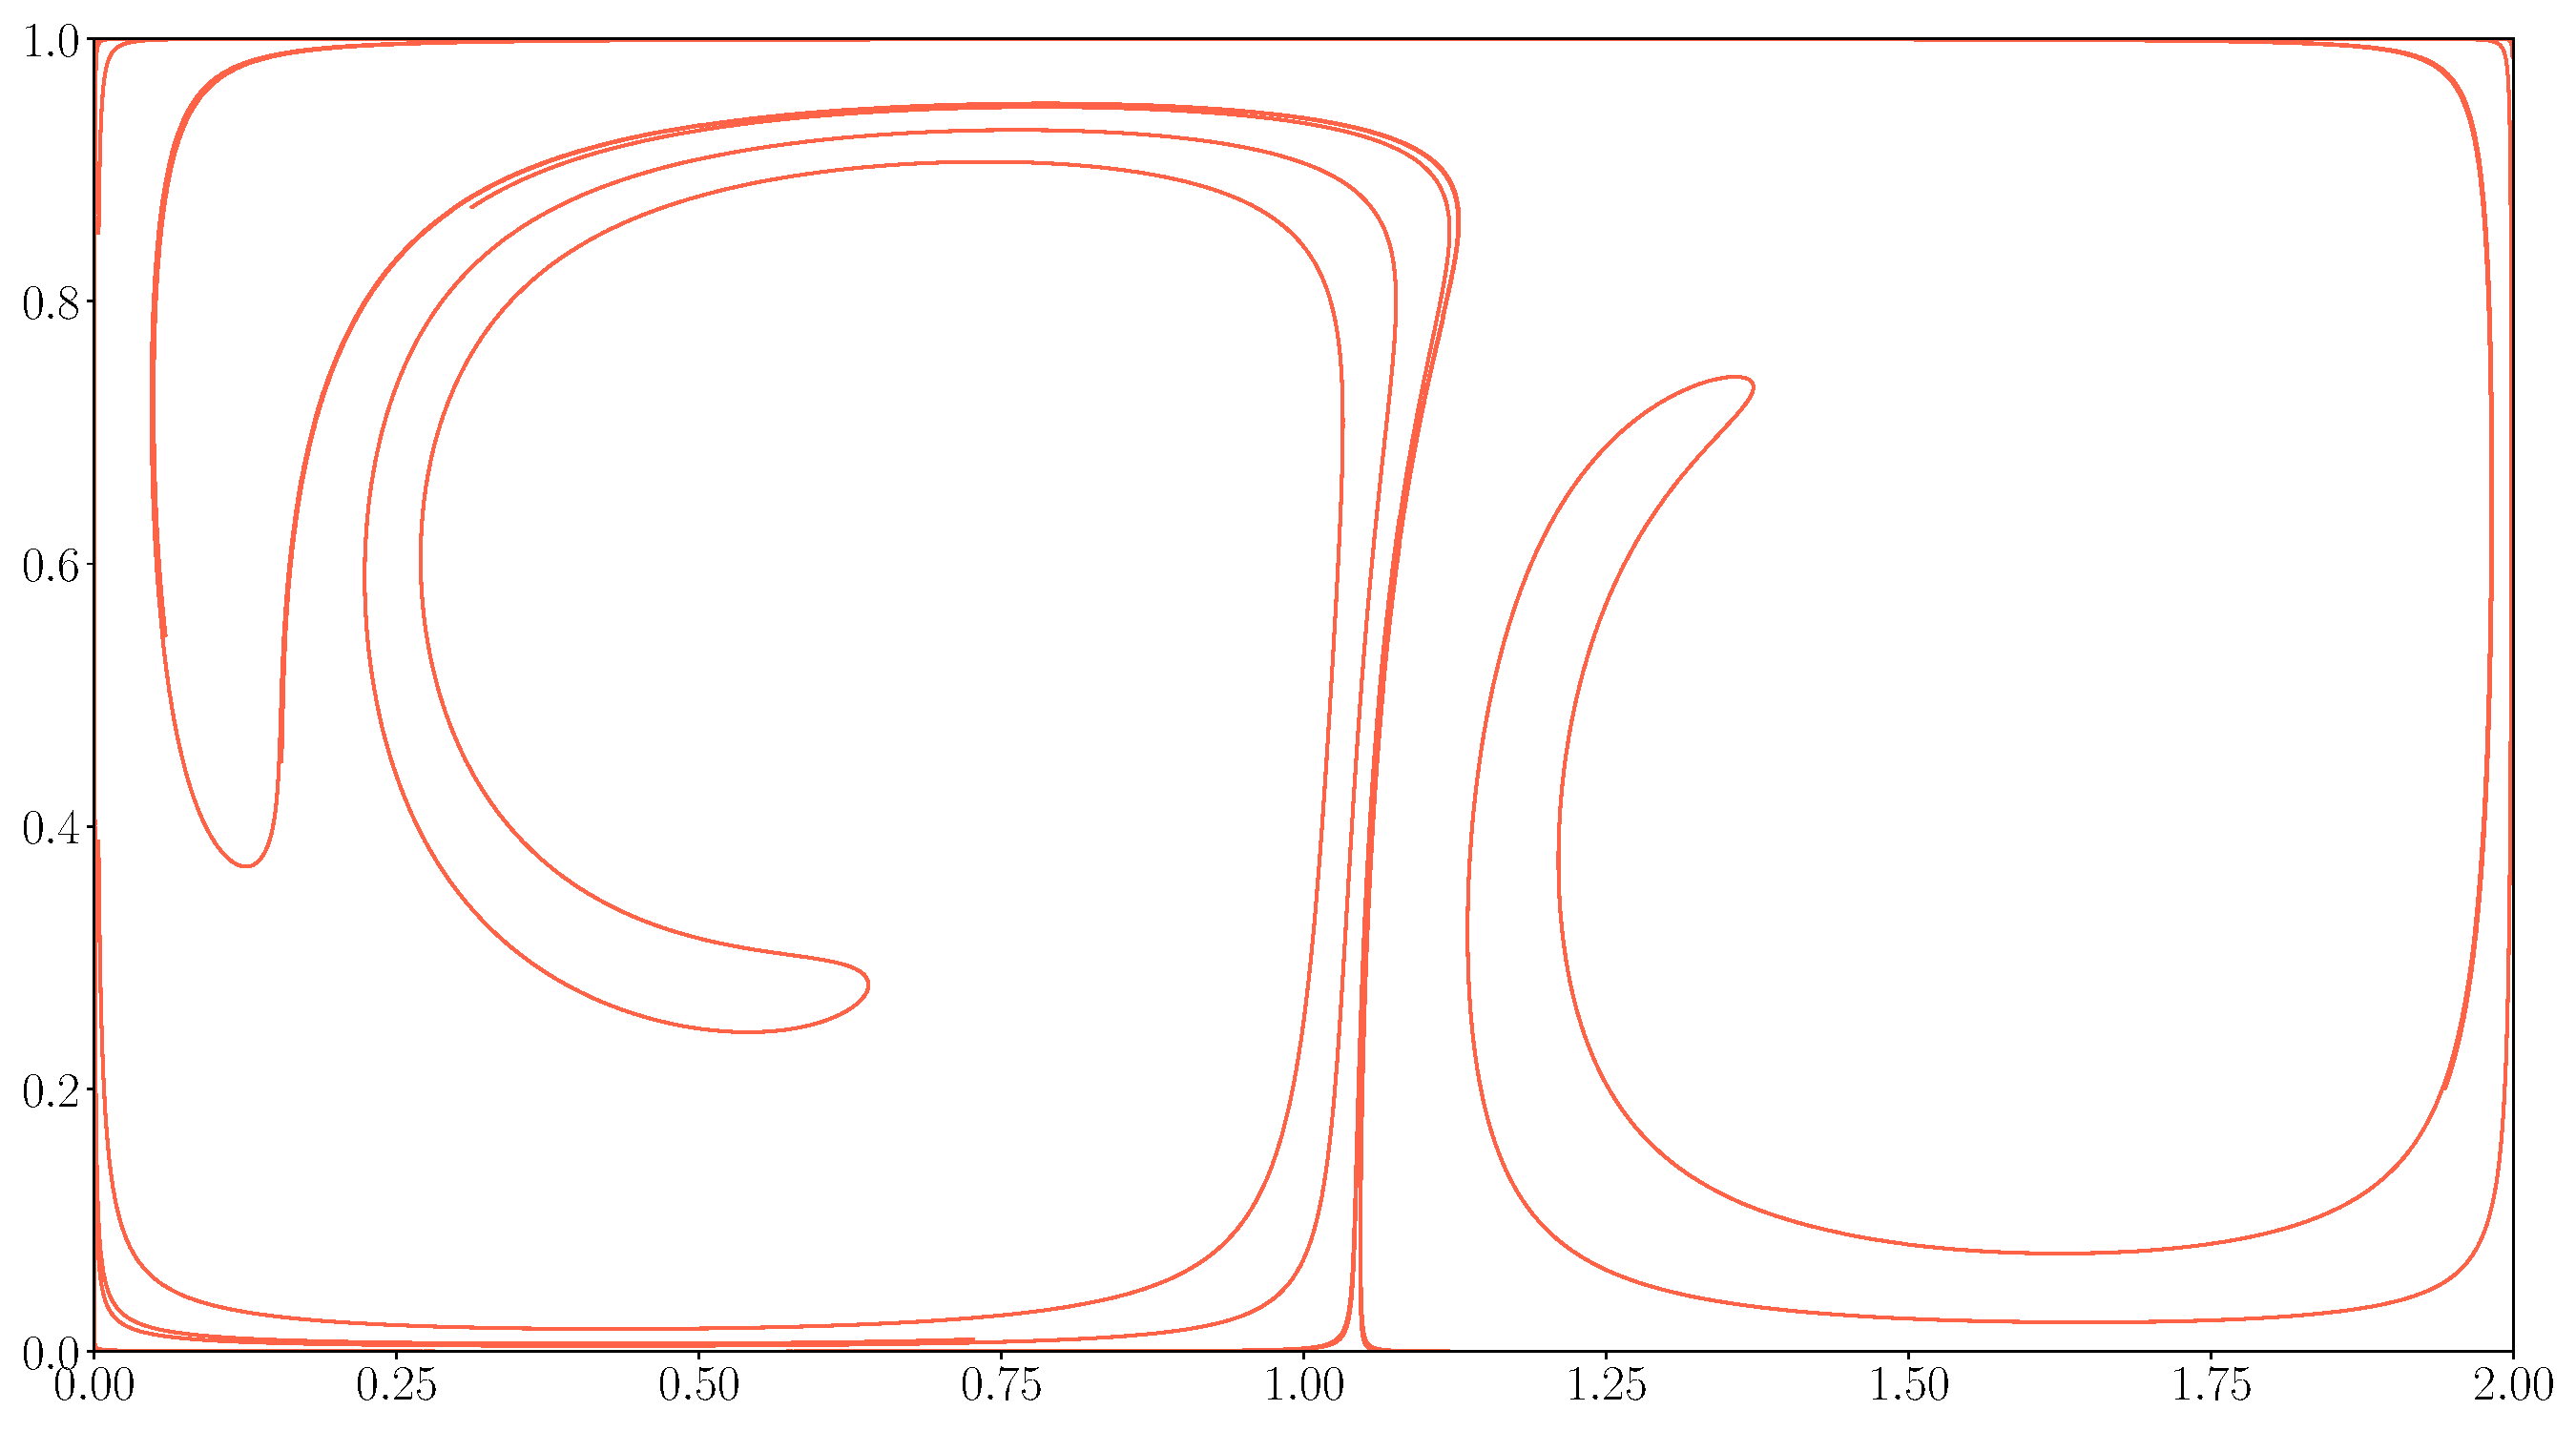
\includegraphics[width=0.9\linewidth]{figures/reference_lcs.pdf}
    \caption[The repelling reference LCS of the double gyre system]{The
    repelling reference LCS of the double gyre system, i.e., the LCS obtained
    by means of the reference numerical integrator, as outlined in
    \cref{sub:on_the_choice_of_numerical_step_lengths_and_tolerance_levels}.
    This curve agrees visually with the LCS found in the literature, for
    instance in \textcite{farazmand2012computing}. It was used as the benchmark
    for comparing the accuracy of the considered numerical integrators,
    outlined in \cref{sub:the_runge_kutta_methods_under_consideration}, for
    varying numerical step lengths and tolerance levels.}
    \label{fig:referencelcs}
\end{figure}
